\documentclass[11pt, a4paper]{article}
\documentclass[spanish, 12pt]{report}
\usepackage[T1]{fontenc}
\usepackage[utf8]{luainputenc}
\usepackage{geometry}
\geometry{verbose,tmargin=2cm,bmargin=2cm,lmargin=2cm,rmargin=2cm,headheight=2cm,headsep=2cm}
\usepackage{float}
\usepackage{textcomp}
\usepackage{amstext}
\usepackage{graphicx}
\usepackage[spanish]{babel}
\usepackage{tikz}
\usepackage[american,oldvoltagedirection]{circuitikz}
\usepackage{amsmath}

\usepackage{relsize}

\begin{document}

\part{Amplificadores de instrumentación}
\section{Introducción}
	Los amplificadores de instrumentación son dispositivos que permiten medir una diferencia de tensión entre sus entradas de forma precisa ya que generan a la salida de los mismos una tensión proporcional a esa diferencia, se utilizan para poder realizar mediciones de precisión sobre pequeñas señales que en otro caso no podrían distinguirse del ruido porque poseen una gran inmunidad frente al mismo.
	
\subsection{Amplificador de diferencias}

\begin{figure}[H]
\centering
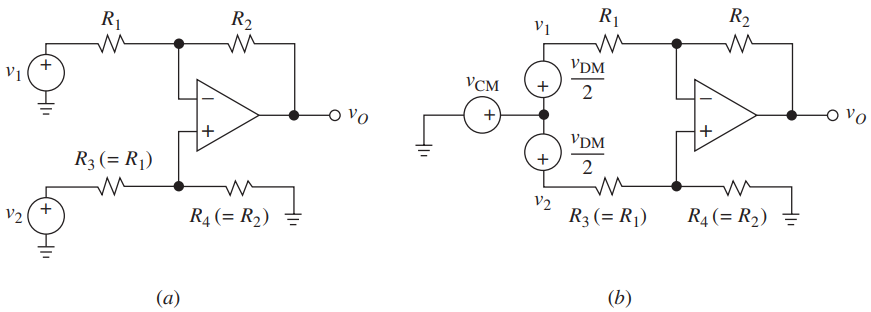
\includegraphics[scale=0.5]{ampdediferencias.png}
\caption{(a) Amplificador de diferencias. (b) Mismo circuito utilizando $V_{CM}$ y $V_{DM}$.}
\label{fig:ampdediferencias}
\end{figure}

	En la Figura $\ref{fig:ampdediferencias}_{(a)}$ se puede observar un amplificador de diferencias típico.
Para apreciar mejor las características del mismo se introducen los componentes de entrada de $\mathit{modo \ diferencial}$ y $\mathit{modo \ comun}$, definidos como:

\begin{equation}
\label{eq:VDM}
V_{DM} = V_2 - V_1
\end{equation}

\begin{equation}
\label{eq:VCM}
V_{CM} = \dfrac{V_1 + V_2}{2}
\end{equation}

	Un amplificador de diferencias ideal responde solamente al componente de modo diferencial $V_{DM}$, e ignora por completo la componente de modo común $V_{CM}$. Para que esto se cumpla se debe de satisfacer la condición de puente balanceado:
	
\begin{equation}
\label{eq:puentebalanceado}
	\dfrac{R_4}{R_3} = \dfrac{R_2}{R_1}
\end{equation}
	
	Obteniendo así la tensión a la salida como:
\begin{equation}
\label{eq:voampdediferencias}
V_O= \dfrac{R_2}{R_1} (V_2 - V_1)
\end{equation}	

	Podemos definir $V_1$ y $V_2$ en función de $V_{CM}$ y $V_{DM}$:
\begin{equation}
\label{eq:V1}
V1=V_{CM} - \dfrac{V_{DM}}{2}
\end{equation}

\begin{equation}
\label{eq:V2}
V2=V_{CM} + \dfrac{V_{DM}}{2}
\end{equation}
	
	Las Ecuaciones \ref{eq:V1} y \ref{eq:V2} ayudan a poder dibujar nuevamente el circuito como se puede ver en la Figura $\ref{fig:ampdediferencias}_{(b)}$.
Se puede observar que quedan definidas como una señal de modo común sobre la cual se sobrepone una señal diferencial. Si se reemplaza en la Ecuación \ref{eq:voampdediferencias} podemos notar nuevamente lo que se ha dicho sobre que si un amplificador de diferencias es ideal, su $V_{CM}$ es cero, cosa que en la realidad es difícil de lograr porque los componentes tienen cierta tolerancia y las condiciones del puente balanceado no serán cumplidas de forma exacta. 

	Resolviendo mediante sustitución y mediante álgebra se puede llegar a:
\begin{equation}
\label{eq:voconganancias}
V_O=A_{DM} \ V_{DM} + A_{CM} \ V_{CM}
\end{equation}

	Donde $A_{DM}$ es la ganancia en modo diferencial y $A_{CM}$ la ganancia en modo común, idealmente la ganancia diferencial debería de ser infinita mientras que la de modo común cero. Utilizando esto podemos definir el CMRR (Razón de rechazo en modo común):
	
\begin{equation}
\label{eq:CMRR}
	CMRR_{dB} = 20 \ \log_{10} \ \abs[\Big]{\dfrac{A_{DM}}{A_{CM}}}
\end{equation}

	Este parámetro permite darse una idea de la capacidad del dispositivo para rechazar las señales en modo común, mientras más alto sea, mejor será el rechazo al modo común.
	
\subsection{Amplificador de instrumentación}
Un amplificador de instrumentación es un amplificador de diferencias que cumple con las siguientes condiciones:
\begin{itemize}
\item[•] Impedancias de entrada de modos diferencial y común extremadamente altas, infinitas para el caso ideal.
\item[•] Impedancia de salida muy baja, cero en el caso ideal.
\item[•] Ganancia estable y precisa.
\item[•] Razón de rechazo de modo común extremadamente alta.
\end{itemize}

\section{Análisis del circuito}
\begin{figure}[H]
\centering
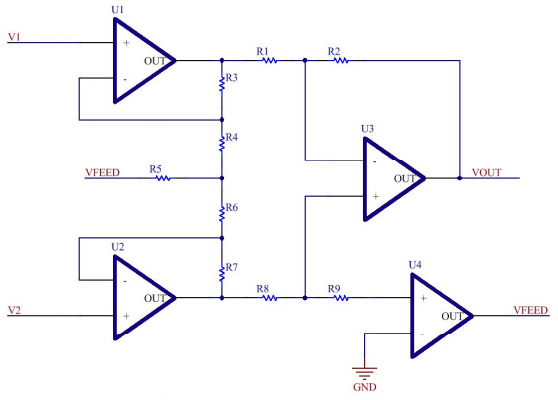
\includegraphics[scale=0.7]{circcatedra.png}
\caption{Circuito propuesto por la cátedra.}
\label{fig:circcatedra}
\end{figure}

\subsection{Caso ideal}
	El amplificador $\mathit{U4}$ en este caso fija una tensión nula en su propia entrada no inversora, su propia salida, en la entrada no inversora del amplificador $\mathit{U3}$ y en la salida del amplificador $\mathit{U2}$.

	El resto del circuito puede ser separado en dos etapas, por una parte tenemos a los amplificadores $\mathit{U1}$ y $\mathit{U2}$ que conforman la etapa de entrada y se encargan de amplificar, además de otorgar a todo el circuito la característica de impedancias de entrada altas, y la etapa de salida conformada por el amplificador $\mathit{U3}$ que teniendo en cuenta lo dicho en el párrafo anterior conforma un amplificador de diferencias con las resistencias $R1 \, , R2 \, , R8$ y $R9$. Un último detalle a mencionar es que se asume que los cuatro amplificadores poseen la misma ganancia $A$.

	Si se calcula $V_{out}$ se obtiene:
\begin{equation}
V_{out} = \dfrac{R_2}{R_1 \, R_4 \, R_7} [R_3 \, (R_6 + R_7) \,V_2 - R_7 \, (R_3 + R_4) \,V_1]
\label{eq:Vout ideal}
\end{equation}
	Para que se encuentre balanceado se necesita entonces que $R_3 \, R_6 = R_7 \, R_4$, obteniendo así:

\begin{equation}
V_{out} = \dfrac{R_2}{R_1} \left( 1 + \dfrac{R_4}{R_3} \right) (V_2 - V_1)
\label{eq:Vout ideal balanceado}
\end{equation}

	Obteniendo así también fácilmente que la $A_{DM}$ es:
	
\begin{equation}
A_{DM} = \dfrac{R_2}{R_1} \left( 1 + \dfrac{R_4}{R_3} \right)
\label{eq:ADM caso ideal}
\end{equation}

	Podemos notar dos cosas, que la ganancia en modo diferencial es la multiplicación de las ganancias de ambas etapas, y que las resistencias $R_5 \, R_6 \, R_7 \, R_8 \, \text{y} \, R_9$ no afectan a la ganancia del mismo en el caso ideal.
	Esto ayuda a poder elegir las resistencias a utilizar a la hora de la implementación del circuito, se deseaba una ganancia de aproximadamente $125 \, dB$, por lo que se eligieron los siguientes valores: $R_1 = 2k \si{\ohm} \, , R_2 = 124.7k \si{\ohm} \, \text{(implementada con dos resistencias en serie)} \, , \text{y} \, R_3 = R_4 = 30.1k \si{\ohm}$. Para seguir manteniendo la igualdad para que se encuentre balanceado, se eligió el mismo valor de $R_3$ y $R_4$ para $R_6$ y $R_7$.

\subsection{Función de R5}
	Mediante simulaciones se fue variando el valor de $R5$ y se observó que no se encontraron diferencias al valor de dicha resistencia en el modo diferencial, mientras que en el modo común esta afectaba gravemente atenuando todas las frecuencias e incluso provocando la aparición de un sobrepico.
	
	Esta resistencia forma parte del lazo de realimentación de un operacional, para ciertos valores esta provocaría que dicha retroalimentación sea positiva y esto se encargará de generar oscilaciones a la salida del sistema.
	
	A la hora de realizar el circuito se utilizó una resistencia de $7.5k\si{ohm}$ ya que se observaba en las mediciones de modo diferencial que funcionaba, sin contemplar el modo común,luego se descubrió que no era un valor óptimo en el momento de las mediciones, en una futura implementación del circuito se agregará o directamente se cambiará esta resistencia por un preset para poder observar los cambios que dichos valores de resistencias provocan en modo común.
	
\section{Implementación del circuito}
	Para las resistencias se utilizaron los valores mencionados anteriormente, se utilizaron resistencias con una tolerancia del 1$\%$ para poder así poder asegurar que se cumple la condición de que este balanceado.
	Para los amplificadores se utilizó el integrado $\mathit{TL084}$ porque este posee una alta impedancia de entrada, un alto valor de Slew Rate que ayuda a evitar problemas al momento de medir la respuesta en frecuencia, y por último pero no menos importante es el hecho de que este integrado tiene 4 amplificadores, lo que hace que sólo necesitemos un integrado para este circuito pero también nos asegura que las ganancias de los mismos sea lo más parecida posible.

\
\section{Respuesta en Frecuencia}
Tanto para las simulaciones como para las mediciones se conecto $V_1$ a un generador y $V_2$ a tierra.
\subsection{Simulacion}
\subsubsection{Montecarlo}

	A continuación se presentan los resultados obtenidos al aplicar las tolerancias de los componentes en la simulación para poder observar como esto podría afectar a la hora de la medición.
	
\begin{center}
	\begin{figure}[H]	
	\makebox[\textwidth]{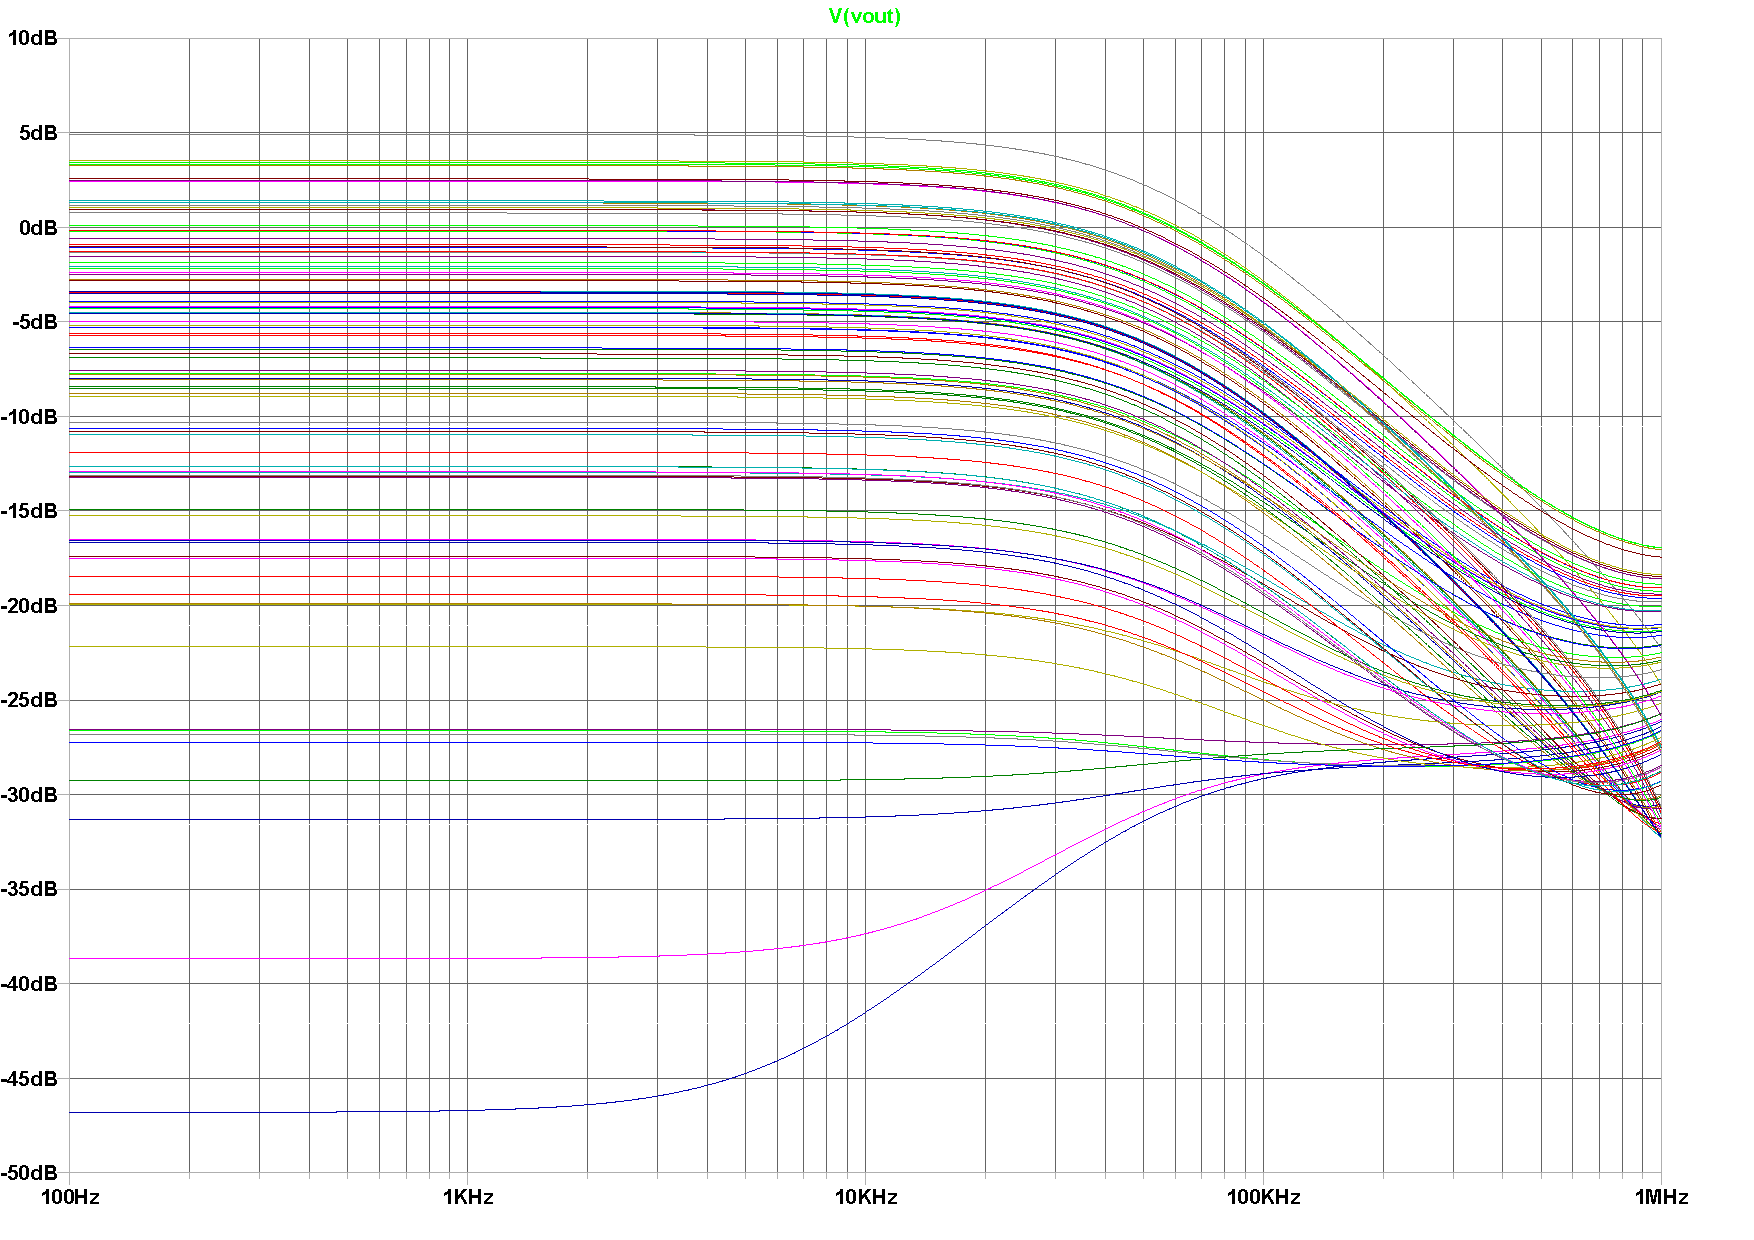
\includegraphics[scale=0.5,keepaspectratio]{ModoCOMunMONTECARLO-MAGNITUD.pdf}}
	\caption{Simulación de montecarlo del modo común en magnitud}
	\label{fig:montecarlodiferencial}
	\end{figure}
\end{center}

	Se puede observar que algunos valores están por encima de $0 \, dB$, lo que nos indica que para algunos casos podría tener una ganancia en lugar de una gran atenuación a frecuencias bajas que es donde se obtiene la ganancia deseada del modo diferencial.

\begin{center}
	\begin{figure}[H]	
	\makebox[\textwidth]{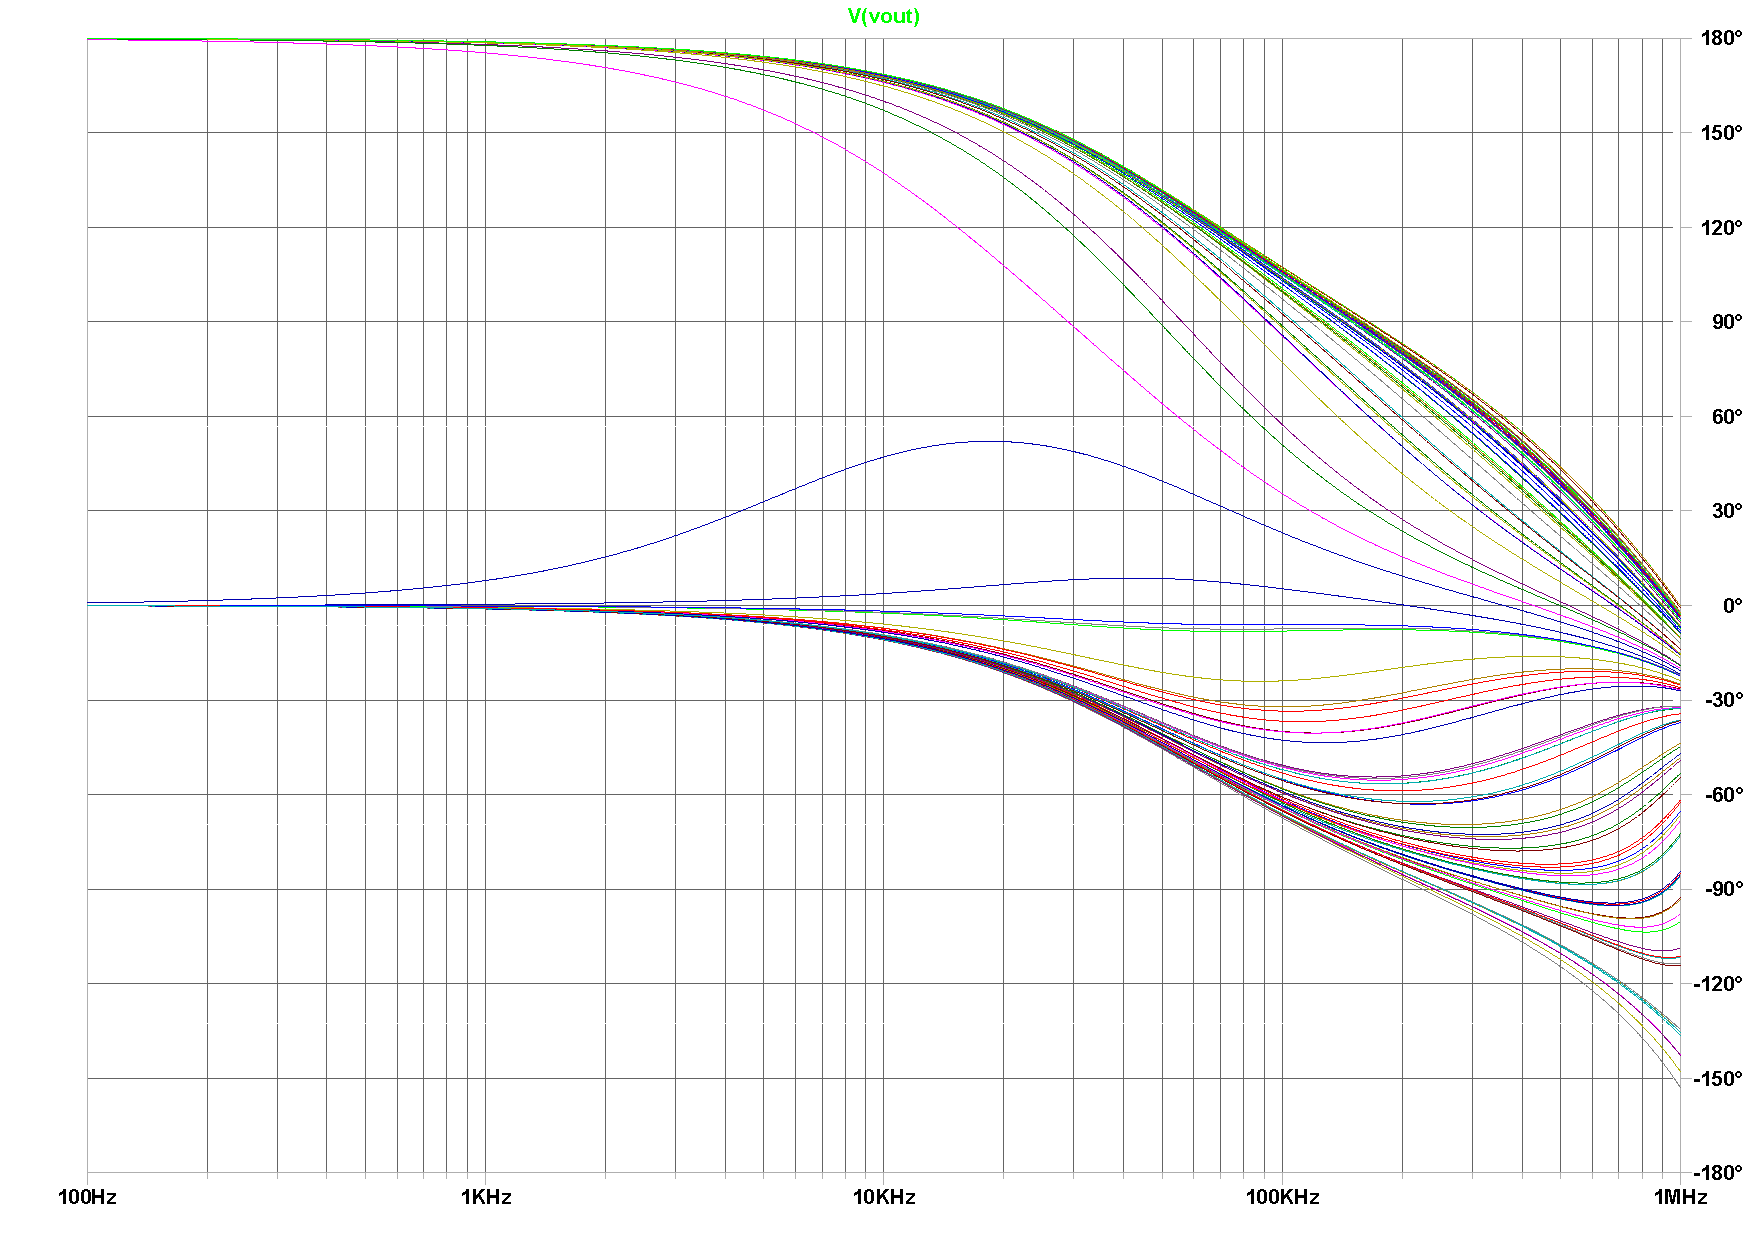
\includegraphics[scale=0.5,keepaspectratio]{ModoCOMunMONTECARLO-FASE.pdf}}
	\caption{Simulación de montecarlo del modo común en fase}
	\label{fig:montecarlodiferencial}
	\end{figure}
\end{center}

\begin{center}
	\begin{figure}[H]	
	\makebox[\textwidth]{\includegraphics[scale=0.5,keepaspectratio]{ModoDIFerencialMONTECARLO.pdf}}
	\caption{Simulación de montecarlo del modo diferencial}
	\label{fig:montecarlodiferencial}
	\end{figure}
\end{center}


\section{Medición}

\begin{figure}[H]
\centering
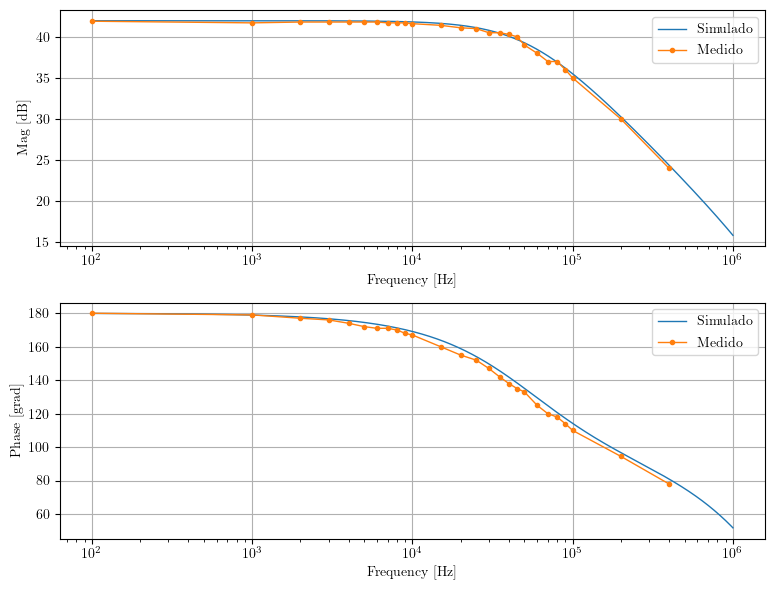
\includegraphics[scale=0.6]{Bode-DIFerencial.png}
\caption{Superposición bode medido y bode simulado para el modo diferencial}
\label{fig:bodemedidodif}
\end{figure}

A la hora de medir el modo diferencial los resultados fueron los esperados y concordaban con gran precisión con lo simulado, esto se debe a que no había grandes cambios de valores en las resistencias que perturbaran el equilibrio balanceado que se busco obtener con la ganancia de modo diferencial.

\begin{figure}[H]
\centering
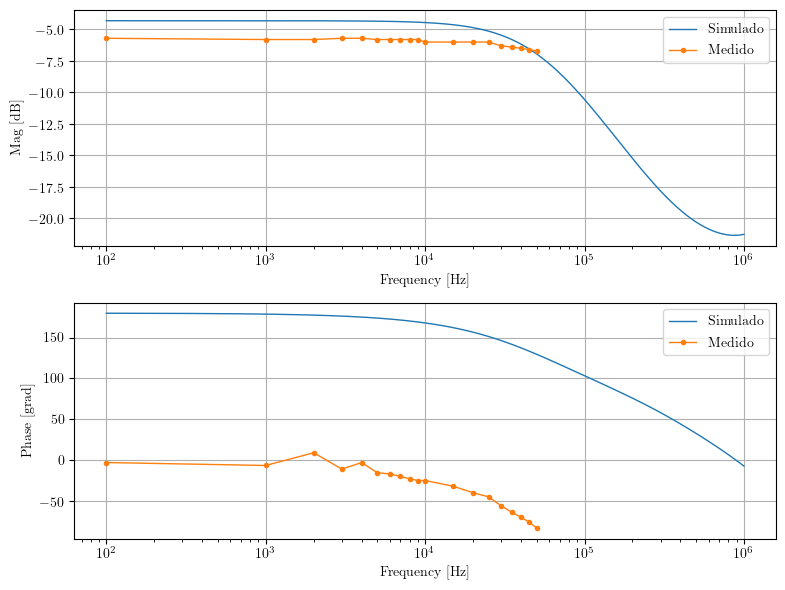
\includegraphics[scale=0.6]{Bode-COMun.png}
\caption{Superposición bode medido y bode simulado para el modo común}
\label{fig:bodemedidocomun}
\end{figure}

	Las mediciones para este modo resultaron no ser iguales a las simuladas cuando no se tiene en cuenta la tolerancia de los componentes, pero se puede notar que pertenecen a una de las curvas de la simulación de montecarlo, mostrando también que no se logró el cometido de obtener $0 \, V$ en modo común
	
\section{Puente de Wheatstone}

\begin{figure}[H]
\centering
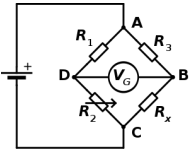
\includegraphics[scale=0.6]{puente.png}
\caption{Puente de Wheatstone}
\label{fig:puente}
\end{figure}

	El puente de Wheatstone es un circuito resistivo que se utiliza para medir el valor de una resistencia desconocida con mucha precisión.
	En la Figura \ref{fig:puente} podemos ver el esquema del puente, siendo $R_x$ la resistencia que se quiere determinar y $R_1, \, R_2, \, \text{y} \, R_3$ resistencias con valores conocidos, siendo $R_2$ una resistencia variable. Se dice que el puente está en equilibrio cuando se cumple que la diferencia entre $V_D$ y $V_B$ es cero, se obtiene así:
	
\begin{equation}
\dfrac{R_2}{R_1} = \dfrac{R_x}{R_3}
\label{eq:EqPuente}
\end{equation}
	
	Donde podemos despejar $R_x = \dfrac{R_2 \, R_3}{R_1}$.
	
\subsection{Generación de señales}
	Se puede notar que la condición de equilibrio del puente es independiente de la tensión que se le aplica al mismo, no importando si esta es continua o de alterna.
	Lo que se busca con este circuito es tener el puente desbalanceado para así poder obtener una diferencia de tensión entre $V_D$ y $V_B$, de forma de alimentar al amplificador de instrumentación con dicha diferencia.
	Mediante divisor resistivo podemos obtener:
\begin{equation}
	V_D= \dfrac{R_2}{R_1+R_2} \, V_A \, , \, V_B = \dfrac{R_3}{R_3+R_4} \, V_A
\end{equation}

	Cumpliéndose estas condiciones se logra que las señales V1 y V2 tengan diferencia
de tensión, obteniendo así una tensión diferencial y que el promedio de ambas tenga un cierto offset con respecto a la masa del circuito, lo cual determina una tensión común. 
	
	En nuestro caso se eligieron los cuatro valores de resistencias iguales, siendo estas de $10k\si{ohm}$  con una tolerancia del $1\%$y se conecto a $R_2$ un preset de 1k, se eligió de esta manera para establecerse en el caso óptimo de puente balanceado y obtener la señal diferencial deseada mediante la modificación del valor del preset.
	
	No se adjunta foto de la medición ya que la misma no aporta nada al análisis ya que la misma muestra una atenuación de la salida del puente de Wheatstone que ya de por si es pequeña, se atribuye esto a un error humano a la hora de la medición (posible mal conexión) ya que se encontraba conectado en modo diferencial, por lo que no debería de atenuar, se buscará tomar una nueva medición y de no ser el caso del error humano, investigar y solucionar este problema.
	
\subsection{Señales no referidas a tierra}
	Si se alimenta al circuito con una señal que no se encuentra referida a la misma tierra, se dice que esta está "flotando" con respecto a la referencia a tierra del circuito. Al existir una diferencia de tensión que desconocemos, si esta toma determinados valores podría ocasionar que nuestra salida del circuito sature, agrega un ruido no deseado a la salida y afecta a la retroalimentación que aportaba el amplificador $\mathit{U_4}$ haciendo que esta deje de funcionar correctamente.







\section{Modificación para obtener una tensión de salida montada sobre un nivel de DC}
	Si la entrada no inversora del operacional $\mathit{U4}$ no se encuentra conectada directamente a tierra, y en cambio se encuentra conectada a una tensión que llamaremos $V_3$, se obtiene:
	
\begin{equation}
V_{out} = \dfrac{R_2}{R_1 \, R_4 \, R_7} [R_3 \, (R_6 + R_7) \,V_2 - R_7 \, (R_3 + R_4) \,V_1] + V_3 \, \left( 1 + \dfrac{R_2}{R_1} - \dfrac{R_2 \, R_3 \, R_6}{R_1 \, R_4 \, R_7}\right)
\label{eq:voconV3}
\end{equation}

\begin{equation}
V_{out} = V_{out,V^+U4aGND} +  V_3 \, \left( 1 + \dfrac{R_2}{R_1} - \dfrac{R_2 \, R_3 \, R_6}{R_1 \, R_4 \, R_7}\right).
\end{equation}
	
	Podemos notar en la Ecuación \ref{eq:voconV3} que se suma un término a la tensión que ya conocíamos de la ecuación \ref{eq:Vout ideal balanceado}, pero debemos recordar que para esta ecuación se encontraba balanceado el circuito mediante la igualdad de resistencias, si aplicamos eso a la ecuación escrita anteriormente obtenemos $V_{out,V^+U4aGND} +  V_3$, por lo que para poder montar la salida sobre una $V_{offset}$ sólo es necesario intercambiar la conexión de GND del amplificador $\mathit{U4}$ a la tensión deseada.
	Esta modificación no se realizó al circuito a la hora de las mediciones pero se agregará para una posterior implementación para su presentación, donde se podría utilizar un preset para así tener un divisor resistivo y poder manejar de esta manera la $V_{offset}$ que se desee.
	
\end{document}
